\chapter*{Búsqueda en profundidad}
\markboth{Búsqueda a profundidad (DFS)}{Búsqueda en profundidad (DFS)}
\addcontentsline{toc}{chapter}{Búsqueda en profundidad (DFS)}

La búsqueda en profundidad, o DFS por sus siglas en ingles, es una búsqueda para ver si existe una solución tomando una serie de operaciones o decisiones. Es muy similar a la búsqueda completa que vimos en la pagina \pageref{decision}, pero es una versión optimizada de esa técnica.

La idea es ir explorando todas las decisiones, pero si una serie de decisiones nos llevan al mismo lugar, ya no volver a explorar por allá. Es decir, la diferencia entre la búsqueda exhaustiva y la DFS, es que esta si detecta que no necesita explorar un lugar que ya fue revisado previamente, no lo hace.

El código de una DFS en general se verá de la siguiente forma:

\begin{lstlisting}
	void DFS(estado) {		
		if (estado fue visitado)
			return;
		marca el estado como visitado;
		for (transiciones del estado) {
			DFS(transicion);
		}
	}
\end{lstlisting}

Veamos un problema ejemplo:

\section*{Ejemplo 4.1}
\addcontentsline{toc}{section}{Ejemplo 4.1}
Javier tiene una calculadora un poco peculiar. Esta tiene un entero \(x\) en la pantalla y dos botones.
\begin{plimits}
	\item El primer botón, al ser presionado le suma \(a\) al número \(x\).
	\item El segundo botón, al ser presionado le suma \(\frac{x}{b}\) a \(x\),  este botón solo puede ser usado cuando \(x\) es múltiplo de \(b\).		
\end{plimits}

Conociendo \(a\) y \(b\), determina si de el valor inicial de \(x\), se puede llegar a tener el número \(y\) en la calculadora.

Además, si se puede imprime como.

\subsection*{Entrada}
Recibes cuatro enteros \(x\), \(y\), \(a\) y \(b\). El valor inicial de la calculadora, el valor deseado, el valor de a, y de b; respectivamente.

\subsection*{Salida}
Si es imposible convertir \(x\) en \(y\), deberás imprimir \verb|NO|.

Si es posible, deberás imprimir un entero \(K\) representando en cuantos pulsaciones de botón lo puedes hacer.

En la siguiente línea imprimirás \(K\) enteros, siendo las pulsaciones a los botones que debes hacer en orden de izquierda a derecha. Un \verb|1| es presionar el primer botón, y un \verb|2| representa el segundo botón.

Si hay varias respuestas, imprime cualquiera. (Ojo: no necesitas minimizar \(K\)).
\subsection*{Ejemplo}
\begin{casebox3}
	\ecase{
		1 20 4 5
	}{
		6\\
		1 2 1 2 1 1
	}{
		Presiona el primer botón, ahora tienes 5.\\		
		Usa el segundo, ahora vale 6.\\
		Pulsa el primer botón, obtienes 10.\\
		Utiliza el segundo para tener 12.\\
		Usa el primer botón, obtén 16.\\
		Termina con el primero, llegamos a 20.
	}
	\ecase{
		1 32 3 2
	} {
		NO
	}{
		Es imposible obtener 32.
	}
\end{casebox3}

\subsection*{Límites}
\begin{plimits}
	\item \(1\leq x, y, a, b \leq 10^5\)
\end{plimits}

TODO ENLACE

\section*{Solución}

Iniciemos con la fuerza bruta.

Podemos ver que cada paso tenemos que tomar dos decisiones, o usamos el botón 1 o el 2. Podemos hacer una búsqueda exhaustiva para ver cual decisión tomar.

\begin{lstlisting}
	void exhaustiva(int x, int pasos) {
		if (x==y) {
			cout << pasos<<"\n";
			for (int i =0; i <pasos; i++) {
				cout<<solucion[i]<<" ";
			}			
			exit(0);
		}
		if (x>y) {
			//x solo crece, de aqui ya es imposible hallar a y.
			return;
		}
		//presiona el boton 1.
		solucion[paso]=1;
		exhaustiva(x+a; pasos+1);,
		
		//presiona el boton 2 si es posible.
		if (x%b==0) {
			solucion[paso]=2;
			exhaustiva(x+x/b, pasos+1);
		}
	}

	int main() {
		[...]
		exhaustiva(0,0);
		cout << "NO";
	}
\end{lstlisting}

Sin embargo, como ya hemos visto, la complejidad de la búsqueda exhaustiva es exponencial, por lo que no correrá para los límites de \(10^5\) que pide este problema. 

Pero, ahora dibujemos lo que hace la búsqueda exhaustiva en el primer caso para ver si podemos mejorarlo.

\begin{center}
	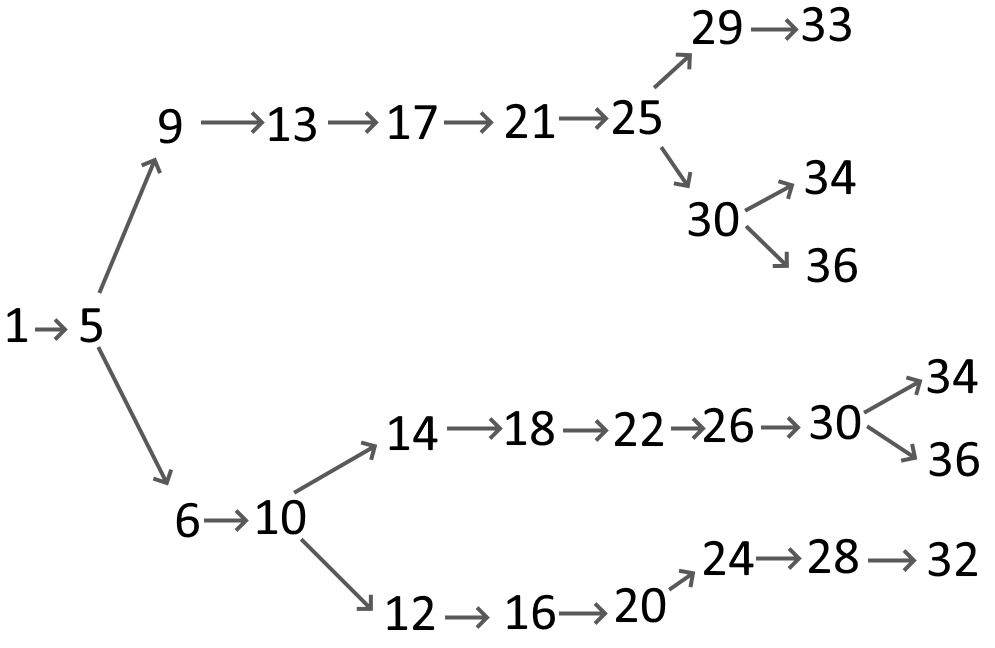
\includegraphics[scale=0.3]{exhaustivaDFS1}
\end{center}

Allí vemos que podemos llegar al 30 con dos rutas. Pero sin importar cual ruta sigamos, de allí solo podemos llegar a los mismos números, al 34 y al 36.

Por lo tanto pregunto ¿realmente tiene sentido la segunda vez revisar el 30?

No, no lo tiene. Al llegar por segunda vez podemos detener la búsqueda, pues ya hemos visto todas las opciones del 30 antes, lo cuál nos ahorrará operaciones.

Ahora nuestra recursión se vería:

\begin{center}
	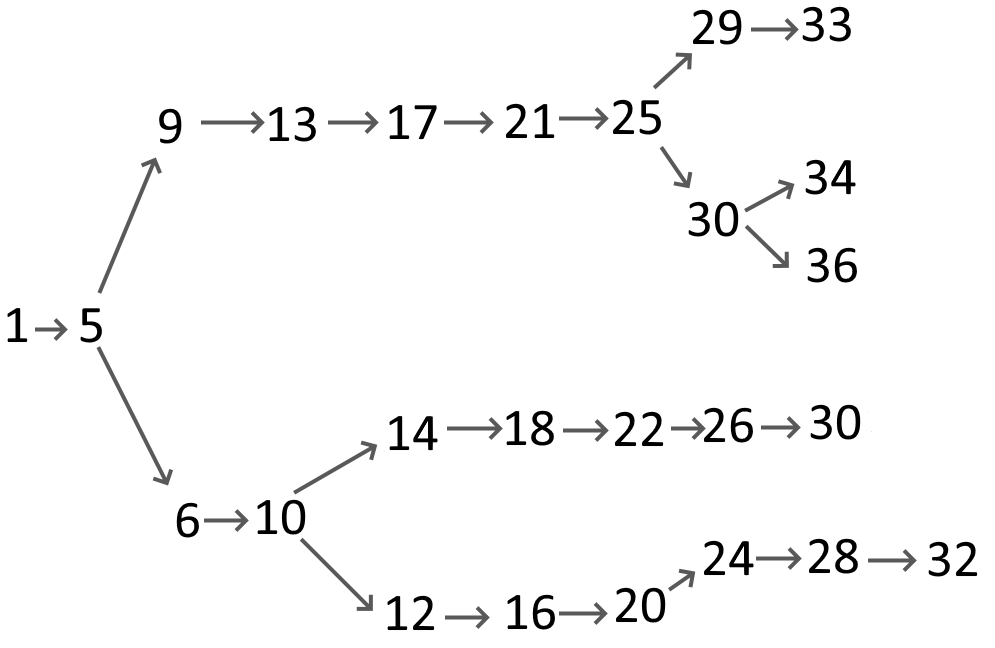
\includegraphics[scale=0.3]{exhaustivaDFS2}
\end{center}

Puede que esto no se vea impresionante en el primer caso ejemplo, pero en el segundo caso ejemplo sí evitamos explorar mucho. Con esta regla, en el segundo ejemplo pasamos de 88 llamadas a la recursión a solo 31.

Entonces, para aplicar la nueva regla podemos tener un arreglo de booleanos llamado \verb|visitado| que lleve cuenta de cuales valores ya visitamos con la búsqueda.

Cuando visitemos un valor de \(x\) revisamos si fue visitado antes, si lo fue detenemos la recursión, si no marcamos a \(x\) como visitado y continuamos con la búsqueda.

Esto en código se ve como:
\pagebreak
\begin{lstlisting}
	bool visitado[100005];
	void busqueda(int x, int pasos) {
		if (x==y) {
			cout << pasos<<"\n";
			for (int i =0; i <pasos; i++) {
				cout<<solucion[i]<<" ";
			}			
			exit(0);
		}
		if (x>y) {
			//x solo crece, de aqui ya es imposible hayar a y.
			return;
		}
		if (visitado[x]) {			
			return;
		}
		//presiona el boton 1.
		solucion[paso]=1;
		busqueda(x+a; pasos+1);,
		
		//presiona el boton 2 si es posible.
		if (x%b==0) {
			solucion[paso]=2;
			busqueda(x+x/b, pasos+1);
		}
	}
	
	int main() {
		[...]
		busqueda(0,0);
		cout << "NO";
	}
\end{lstlisting}

Y tal cual, esto es una DFS, una búsqueda que va probando todas las opciones de donde se encuentra actualmente, pero nunca repitiendo la búsqueda en lugares ya visitados.

Analicemos la complejidad de este algoritmo, aquí es donde esta lo genial de este tema.

Veamos que este código solo ejecuta la parte de probar al botón 1 y 2 una sola vez por cada valor de \(x\) posible.

Y la parte de arriba solo es ejecutada tantas veces como búsqueda sea llamada(), que ya vimos que esta limitada a los posibles valores de \(x\).

Como nuestros valores de \(x\) varían desde \(1\) hasta \(y\), la complejidad de este algoritmo es \(O(y)\). Lo cual significa que pasamos de un algoritmo exponencial a uno lineal. He aquí la hermosura de la búsqueda en profundidad, o DFS.

\section*{Estados y transiciones}
\addcontentsline{toc}{section}{Estados y transiciones}
Hasta ahorita este libro ha sido un poco informal en como le llama a "decisiones/lugares" que son alcanzables con las "opciones".

En el ejemplo 4.1 teníamos como "lugar", el número \(x\) y las "opciones" eran presionar el botón 1 o el botón 2.

Pero ahora vamos a ser un poco más formales y darles el nombre correcto y debido a esto. 

Los lugares a los que llevamos, donde tenemos que tomar decisiones que los representamos con argumentos en la función recursiva, el nombre que usaremos ahora es estado. Es decir, es un estado de la búsqueda a la cual puedes llegar después de tomar varias "opciones".

Y a las "opciones" que tomamos, que nos mueven de un estado a otro y que son las llamadas recursivas que hacemos les pondremos de nombre formal "transiciones".

Entonces, nuestra búsqueda DFS explora todos los estados alcanzables desde uno inicial, utilizando las transiciones disponibles.
\section*{Complejidad}
\addcontentsline{toc}{section}{Complejidad}
La complejidad de una DFS es la cantidad de estados más transiciones, llamemos al número de estados \(V\) y \(E\) al número de transiciones total. La DFS corre en \(O(V+E)\).

En el ejemplo 4.1 teníamos \(y\) estados, así como a lo más \(2y\) transiciones (dos por cada estado de los botones), la complejidad del ejemplo es pues: \(O(V+E)=O(y+2y)=O(y)\).



\newpage

\practiceproblemsection{4}

\problembreak

\problemtitle Te encuentras en una torre que tiene \(N\) pisos enumerados del \(1\) al \(N\).

El piso \(i\) tiene \(P_i\) pasadizos, cada pasadizo te permitirá moverte a un piso superior desde \(i\). Los pasadizos no se puede usar para bajar.
Ademas, el ultimo piso no tiene pasadizos.

Desgraciadamente, habrá veces en que te sea imposible viajar del piso \(1\) al piso \(j\) debido a como fueron construidos los pasadizos.

Ahora, dado la descripción de los pisos, determina a cuantos pisos puedes alcanzar desde el piso 1.
\subsubsection*{Entrada}
Dos enteros \(N\), la cantidad de pisos en la torre.

En las siguientes \(N-1\) lineas vendrá la descripción de cada piso. 

Cada piso constará de un entero \(P_i\) representando cuantos pasadizos hay allí que conectan hacia arriba. Seguido, vendrán \(P_i\) enteros diferentes, representando a que pisos tienes un pasadizo. Solo habrá pasadizos a pisos superiores.

\subsubsection*{Salida}
Imprime un entero que represente la cantidad de pisos que son alcanzables desde el primero.

\subsubsection*{Ejemplo}
\begin{casebox3}
	\ecase{
		10\\
		3 2 5 7\\
		1 3\\
		0\\
		2 4 5\\
		1 7\\
		3 6 8 10\\
		1 10\\
		0\\
		2 9 10\\
		9 10		
	}{5}{
	Podemos visitar los pisos:\\
	1, 2, 3, 5 y 7.
	}
\end{casebox3}

\subsubsection*{Límites}
\begin{plimits}
	\item \(1\leq N\leq 5\times10^4\)
	\item \(0\leq P_i\leq 10\)
\end{plimits}
\subsubsection*{Subtareas}
\begin{plimits}
	\item (45 puntos) \(1\leq N\leq 12\)
	\item (55 puntos) \(1\leq N\leq 5\times10^4\)
\end{plimits}

ENLACE: TODO

\problemtitle Javier esta en un tablero de \(N\) filas y \(M\) columnas. En este tablero habrá unas celdas libres y unas celdas bloqueadas.

Él se encuentra en la casilla superior izquierda, la \((1, 1)\), y quiere llegar a la casilla \((f,c)\). La casilla donde Javier inicia siempre será libre.

Javier puede en cualquier momento, dar un paso y moverse a cualquiera de las cuatro casillas de arriba, abajo, izquierda o derecha. Siempre y cuando estas casillas existan y no estén bloqueadas. 

Determina si existe un camino de donde esta Javier a donde quiere ir.

\subsubsection*{Entrada}
Dos enteros \(N\) y \(M\), el número de filas y el número de columnas del tablero.

En las siguientes \(N\) líneas recibirás \(M\) caracteres, siendo la descripción del tablero. '\#' simboliza una casilla bloqueada y '.' es una libre.

En la última línea tendrás dos enteros. \(f\) y \(c\), la fila y columna donde esta la celda a la que Javier quiere ir.

\subsubsection*{Salida}
Imprime \verb|SI| en caso de que exista un camino de \((1, 1)\) a \((f, c)\). De lo contrario imprime \verb|NO|.

\subsubsection*{Ejemplo}

\begin{casebox3}
	\ecase{
		3 5\\
		\texttt{..\#.\#}\\
		\texttt{\#...\#}\\
		\texttt{..\#\#.}\\
		3 1
	} {
	SI
	}{
	\\
	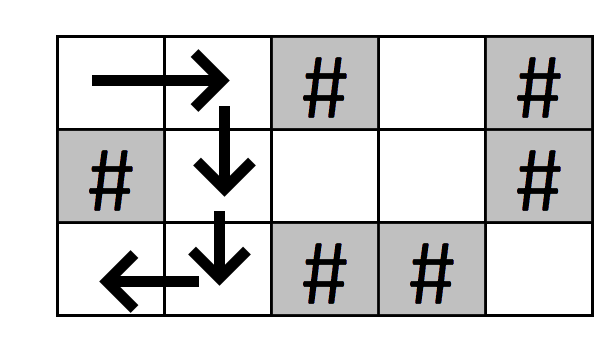
\includegraphics[scale=0.20]{caminoDFS1}
	}
	\ecase{	
		4 5\\
		\texttt{....\#}\\
		\texttt{\#...\#}\\
		\texttt{\#.\#\#.}\\
		\texttt{...\#.}\\
		3 5\\
	}{NO}{}
\end{casebox3}

\subsubsection*{Límites}
\begin{plimits}
	\item \(2\leq N, M\leq 1000\)
	\item \(1\leq f \leq N\)
	\item \(1\leq c \leq M\)
\end{plimits}

\omegalink{} TODO